\chapter{Revis�o de Literatura} 
\label{capitulo:revisao}


\section{Steering Behaviors}

Com o objetivo de criar uma solu��o para ~\cite{reynolds-99-steering} so pode ~\ref{fig:steer_separation} \ref{fig:steer_alignment}
\ref{fig:steer_cohesion}

Desenvolvido por Reynolds em 1986 ~\cite{reynolds-99-steering} como proposta de um modelo baseado em for�as para tratar comportamento de movimenta��o em grupo, como: cardumes, enxames, manadas e outros. O modelo b�sico consistem em tr�s simples for�as conhecidas como {\it steering behaviors} as quais direcionam os elementos do grupo individualmente baseado na velocidade e posi��o dos elementos vizinhos, essas for�as s�o: separa��o, alinhamento e coes�o e podem ser vistas nas figuras ~\ref{fig:steer_separation} \ref{fig:steer_alignment}
\ref{fig:steer_cohesion} respectivamente.

{\it it�lico}
{\bf negrito}
{\tt c�digo}

\begin{figure}
\centering
\resizebox{5cm}{!}{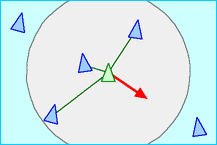
\includegraphics{figuras/steer_separation.png}}
\caption{Separa��o: {\it Steer} para evitar o agrupamento com elementos vizinhos}
\label{fig:steer_separation}
\end{figure}

\begin{figure}
\centering
\resizebox{5cm}{!}{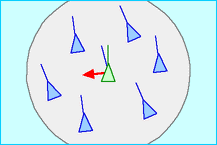
\includegraphics{figuras/steer_alignment.png}}
\caption{Alinhamento: {\it Steer} com objetivo de alinhar o elemento com seus vizinhos}
\label{fig:steer_alignment}
\end{figure}

\begin{figure}
\centering
\resizebox{5cm}{!}{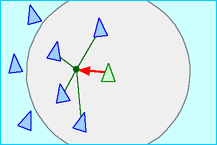
\includegraphics{figuras/steer_cohesion.png}}
\caption{Coes�o: {\it Steer} de agrupamento com os elementos vizinhos}
\label{fig:steer_cohesion}
\end{figure}

Falar sobre reinolds, boids, birds e afins.
\subsection{Mec�nica}
- Funcionamento e objetivo dos steerings.
\subsection{Aplica��es}
- Utiliza��es (citar outras utiliza��es al�m de direcionamento de elementos)

\section{Simula��o de fluidos}
Formas de simula��o de fluidos
\subsection{Baseadas em Malha (Eulerian)}
Stable fluids 
\subsection{BBaseadas em Part�culas (Lagrangian)}
SPH (smoothed particle hydrodynamics)